\justify{}
\textcopyright{} 2021, by Franklin Diaz
\justify{}
Licensed under \href{https://creativecommons.org/licenses/by-nc-nd/4.0/}{CC BY-NC-ND 4.0} 
\faCreativeCommons\ \faCreativeCommonsBy\ \faCreativeCommonsSa\
\vspace{5mm}\\
First Edition 2021
\justify{}
Front cover image design by {\href{https://www.linkedin.com/in/eddiemize/}{Eddie Mize}}.
Images at the beginning of the chapters in this book are
\href{https://pixabay.com/service/terms/#license}{courtesy of Pixabay}
\justify{}
The source for this book is available from 
{\href{https://github.com/thedevilsvoice/devsecops\_tactical\_book}{devsecops\_tactical\_book}}
\vspace{3mm}
Published on: \today
\justify{}
This book was initially drafted using the reStructuredText file format.
The Sphinx module for Python was used to format these files and programatically
generate LaTeX, and other working formats used in the typesetting process. The
resultant LaTeX files were managed using TeXstudio.
\justify{}
Some graphs have been generated programatically using the Graphviz software.
The entire publishing environment is developed and maintained according
to the principles outlined in this book.
\vspace{5mm}
\centering
\vspace{0mm}
\begin{figure}[!htb]
	\centering
	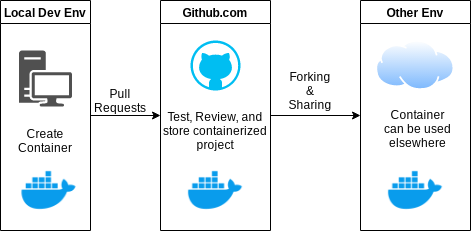
\includegraphics[scale=0.75]{../images/workflow.png}
\end{figure}
\vspace{2mm}
Containerized publishing work flow.
